\chapter{Deadlocks}
Nowadays the OS has more instance of the same resource for example think about to the CPU, normally in 2024, it contains more than 4 core.

Each tasks require a lot of different resources: 

\begin{itemize}
    \item CPU time;
    \item network;
    \item read \& write from the SSD;
    \item etc.
\end{itemize}

and for each the process must: request, use and release the resource. I would to find a general role to check before if it could be a deadlock.

\paragraph{Example: } If we have P1 and P2 and each 2 chopstick, we understood that there will never be a deadlock.

\paragraph{}

Deadlock can arise if four conditions hold simultaneously:


\begin{itemize}
    \item \textbf{Mutual exclusion}: only one thread at a time can use a resource, sharing variable is risky BUT NOT in all cases, only in R/W case!;
    \item \textbf{Hold and wait}: a thread holding at least one resource is waiting to acquire additional resources held by other threads, chopstick;
    \item \textbf{No preemption}: a resource can be released only voluntarily by the thread holding it, after that thread has completed its task;
    \item \textbf{Circular wait}: there exists a set {T0, T1, ..., Tn} of waiting threads such that T0 is waiting for a resource that is held by T1, T1 is waiting for a resource that is held by T2, ..., Tn–1 is waiting for a resource that is held by Tn, and Tn is waiting for a resource that is held by T0. (n > 1)
\end{itemize}

\newpage
\section{Resource-Allocation Graph}


\begin{figure}[htbp]
    \centering
    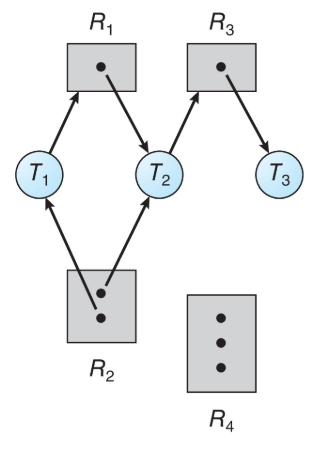
\includegraphics[width=0.25\linewidth]{img/garph.png}
    \caption{Resource Allocation Graph Example}
\end{figure}

One instance of R1, Two instances of R2, One instance of R3, Three instance of R4.


T1 holds one instance of R2 and is waiting for an instance of R, T2 holds one instance of R1, one instance of R2, and is waiting for an instance of R, T3 is holds one instance of R3.

In this situation there are \textbf{none deadlock}, no circular waiting.

\subsubsection{Example of deadlock}

\begin{figure}[htbp]
    \centering
    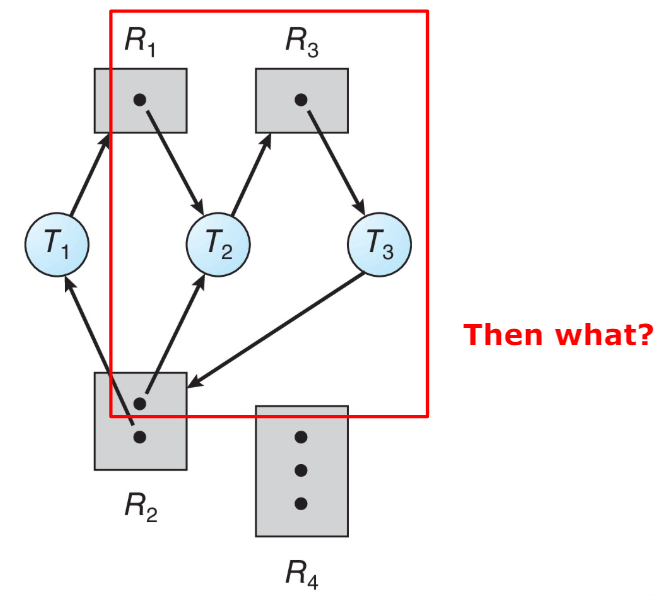
\includegraphics[width=0.4\linewidth]{img/ragWith_dead.png}
\end{figure}

In this case there is a deadlock, because there are two circular wait!


\subsubsection{Example of no deadlock}

\begin{figure}[htbp]
    \centering
    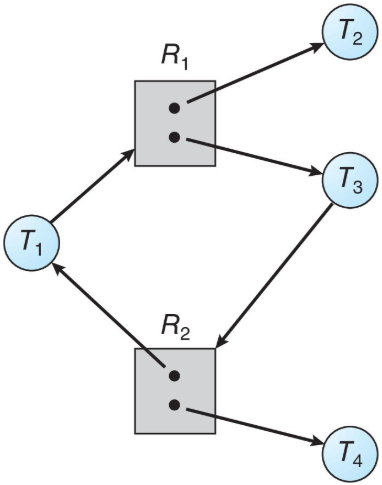
\includegraphics[width=0.27\linewidth]{img/g_no_dead.png}
\end{figure}
No deadlock here, eventually T4 will release R2, making it available to T3 who is requesting it.

\subsubsection{Summary}

\begin{itemize}
    \item If graph contains no cycles $\to$ no deadlock
    \item If graph contains a cycle $\to$
    \begin{itemize}
        \item[] if only one instance per resource type involved, then deadlock
        \item[] if several instances per resource type, possibility of deadlock
    \end{itemize}
\end{itemize}

\section{Methods for Handling Deadlocks}

We want to handle the deadlock that happened. Is difficult for a system recover a deadlock that happened, thus we ensure that the system will never enter a deadlock state:

\begin{itemize}
    \item Deadlock prevention
    \item Deadlock avoidance
\end{itemize}

\section{Deadlock Prevention}

Invalidate one of the four necessary conditions for deadlock:

\begin{itemize}
    \item Mutual Exclusion – not required for sharable resources (e.g., read-only files); must hold for non-sharable resources
    \item Hold and Wait – must guarantee that whenever a thread requests a resource, it does not hold any other resources

    \begin{itemize}
        \item Require threads to request and be allocated all its resources before it begins execution or allow thread to request resources only when the thread has none allocated to it.
        \item Cons: Low resource utilization; starvation possible
    \end{itemize}

    \item No Preemption:

    \begin{itemize}
        \item If a process that is holding some resources requests another
resource that cannot be immediately allocated to it, then all
resources currently being held are released
        \item Preempted resources are added to the list of resources for which
the thread is waiting
        \item Thread will be restarted only when it can regain its old resources,
as well as the new ones that it is requesting
    \end{itemize}

    \item Circular Wait:

    \begin{itemize}
        \item Impose a total ordering of all resource types, and require that each
thread requests resources in an increasing order of enumeration, Not always flexible, but doable
    \end{itemize}
\end{itemize}


\section{Circular Wait}
Invalidating the circular wait condition is most common. Simply assign each resource (i.e., mutex locks) a unique number.

Resources must be \textbf{acquired in order}.
All the process has the same structure like this:

\begin{codeInC}
wait(M1)
wait(M2)

/* execution */

signal(M2)
signal(M1)    
\end{codeInC}
\newpage

\section{Deadlock Avoidance}

Requires that the system has some additional a priori information available.

Simplest and most useful model requires that each thread declare the maximum number of resources of each type that it may need.he deadlock-avoidance algorithm dynamically examines the
resource-allocation state to ensure that there can never be a
circular-wait condition.

Resource-allocation state is defined by the number of available and
allocated resources, and the maximum demands of the processes

\paragraph{}
This is \textbf{feasible in real-time systems}, where tasks have to be
allocated in advance for schedulability evaluation, and also to check for deadlocks.


\section{(Thread-)Safe State}
When a thread requests an available resource, system must decide if immediate allocation leaves the system in a safe state.

System is in safe state if a sequence of thread wanting to execute a task has ALL the necessary resource.

That is:
\begin{itemize}
    \item If Ti resource needs are not immediately available, then Ti can wait until all Tj have finished;
    \item When Tj is finished, Ti can obtain needed resources, execute, return allocated resources, and terminate;
    \item When Ti terminates, Ti +1 can obtain its needed resources, and so on.
\end{itemize}

\section{Recap}

\begin{itemize}
    \item If a system is in safe state $\to$ no deadlocks;
    \item If a system is in unsafe state $\to$ possibility of deadlock;
    \item Avoidance $\to$ ensure that a system will never enter an unsafe state, thus, ensure that there will be no deadlocks!
\end{itemize}

\begin{figure}[htbp]
    \centering
    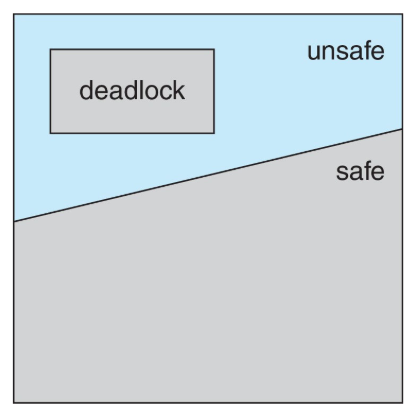
\includegraphics[width=0.3\linewidth]{img/Dead.png}
\end{figure}